% Name: Sorting network
% Description: The five comparators that sort any four values, shown sorting 3, 1, 4, 2.
% Tags: sorting network, comparators, parallel algorithms

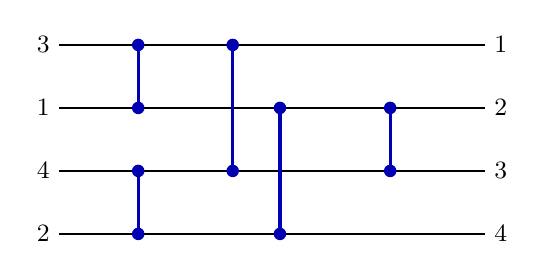
\begin{tikzpicture}[x=1cm, y=8mm, every node/.style={font=\small}]
  \foreach \w/\in/\out in {1/3/1, 2/1/2, 3/4/3, 4/2/4} {
    \draw[thick] (0,-\w) -- (5.4,-\w);
    \node[left] at (0,-\w) {$\in$};
    \node[right] at (5.4,-\w) {$\out$};
  }
  \foreach \x/\a/\b in {1/1/2, 1/3/4, 2.2/1/3, 2.8/2/4, 4.2/2/3}
    \draw[very thick, blue!70!black] (\x,-\a) node[circle, fill=blue!70!black, inner sep=1.6pt] {}
      -- (\x,-\b) node[circle, fill=blue!70!black, inner sep=1.6pt] {};
\end{tikzpicture}
